\documentclass[a4paper,11pt]{article}
\usepackage{lmodern}			% Usa a fonte Latin Modern
\usepackage[T1]{fontenc}		% Seleção de códigos de fonte
\usepackage[utf8]{inputenc}		% Codificação do documento
\usepackage[brazil]{babel}
\usepackage{indentfirst}		% Indenta o primeiro parágrafo de cada seção.
\usepackage{graphicx}			% Inclusão de gráficos
\usepackage{amssymb}
\usepackage{xcolor}
\usepackage{tcolorbox}
\usepackage{subcaption}			% subfiguras (subfig e subfigure removidos: são incompatíveis com o subcaption)
\usepackage{caption}
\usepackage{enumitem}
\usepackage{tikz}
\usetikzlibrary{shapes.geometric,arrows,positioning}
% Definição do símbolo de soma
\tikzset{
    sum/.style = {draw, circle, minimum size=0.5cm, node distance=1cm, inner sep=0pt, label=center:{\tiny $+$}},
    block/.style = {draw, rectangle, minimum height=1cm, minimum width=1.5cm},}
\usepackage[
%	a4paper,
left=2cm,
right=1.5cm,
bottom=1.5cm,
top = 2.5cm,
foot=0.7cm]{geometry}
\usepackage{url}
\usepackage{setspace}
\usepackage{amsmath}
\usepackage{amsfonts}
\usepackage{fancyhdr}

\fancypagestyle{plain}{
    \fancyhf{} % Limpa campos de cabeçalho e rodapé
    %\renewcommand{\headrulewidth}{0pt} % Remove a linha horizontal do cabeçalho
    %\renewcommand{\footrulewidth}{0pt} % Remove a linha do rodapé
   }
\usepackage{multirow}
\usepackage{tabularx}
\usepackage{booktabs}			% \toprule, \midrule, \bottomrule
\usepackage{array}				% tipos de coluna personalizados
\usepackage{float}				% posicionamento [H]
\usepackage{natbib}
\setlength{\headheight}{14.2pt}
\bibliographystyle{abbrvnat}
\setcitestyle{open={(},close={)}}
 %Citation-related commands
\usepackage{hyperref}

\graphicspath{{figuras/}{./}}	% procura as imagens na pasta figuras/ ou na raiz do projeto
\newcolumntype{L}{>{\raggedright\arraybackslash}X}
\newcolumntype{C}[1]{>{\centering\arraybackslash}p{#1}}

\pagestyle{fancy}

\begin{document}
	\onehalfspacing
	\thispagestyle{empty}
\begin{center}
	
\includegraphics[height=2cm]{logoUFSCsimples} \\
	{\large Universidade Federal de Santa Catarina -- UFSC} \\
	{\large Centro Tecnológico -- CTC} \\
	{\large Departamento de Engenharia de Automação e Sistemas -- EAS} \\
	%\vspace{1cm}
	{\large DAS5151 - Instrumentação em Controle} \\
	\vfill
	\textbf{Primeira Entrega do Projeto Final} \\


	\vspace{1cm}

	Autores: \\
    Yuri Melo Nunes (20104163) \\
    Giulia Cenci dos Santos (20202446) \\
    Ana Luíza Luft (20204495) \\
    \vspace{1cm}
    Prof. Rodolfo Cesar Costa Flesch\\


	\vfill
	Florianópolis, \today.
\end{center}

\clearpage

\tableofcontents

\clearpage

\tcbset{colback=gray!10, colframe=white, arc=0mm, boxrule=0pt, left=2mm, right=2mm, top=2mm, bottom=2mm}

% ================= 1 =================
\section{Descrição do projeto}

O projeto consiste no controle da temperatura de uma câmara térmica confinada, construída em poliestireno expandido (EPS) e aquecida por resistores de potência acionados por modulação por largura de pulso (PWM). A temperatura interna é medida por dois termorresistores Pt100 com ligação a 3 fios, montados em uma ponte de Wheatstone cujo sinal é amplificado por um amplificador de instrumentação. A temperatura ambiente, principal perturbação do sistema, é medida por um sensor digital DS18B20 posicionado fora da câmara. Uma ventoinha mantém o ar interno homogêneo, e um Arduino Uno realiza a aquisição dos sinais e a geração do PWM.

Em relação à proposta inicial, foram feitas as seguintes alterações:

\begin{itemize}
  \item \textbf{Medição da temperatura ambiente:} incluída conforme sugerido na avaliação da proposta, para permitir uma compensação antecipativa (\textit{feedforward}) da perturbação. É feita com um sensor DS18B20 fornecido pelo professor.
  \item \textbf{Componentes adequados à disponibilidade do LMM:} o amplificador de instrumentação passou a ser o INA125P, que opera com alimentação única de 5\,V e dispensa fonte simétrica; o acionamento passou a ser feito por um optoacoplador PC817 e um transistor Darlington TIP122; o aquecedor é uma placa com três resistores de potência disponível no laboratório; e os resistores e o diodo do circuito foram escolhidos entre os valores disponíveis.
  \item \textbf{Ligação a 3 fios:} adotada a configuração em que um dos fios do par de cada Pt100 leva o sinal até o amplificador, conforme orientação do professor (Seção~\ref{sec:pt100}).
  \item \textbf{Realimentação de corrente:} a medição de corrente por resistor \textit{shunt} prevista na proposta foi retirada nesta etapa. O optoacoplador isola o circuito de potência do microcontrolador, e a medição da corrente exigiria compartilhar novamente as referências de terra. A medição poderá ser reavaliada nas próximas etapas.
\end{itemize}

% ================= 2 =================
\section{Premissas de projeto}

\begin{itemize}
  \item \textbf{Faixa de setpoint:} da temperatura ambiente até cerca de 50\,\ensuremath{^\circ}C, abaixo da temperatura em que o EPS começa a amolecer (cerca de 80\,\ensuremath{^\circ}C).
  \item \textbf{Faixa de medição interna:} aproximadamente 12\,\ensuremath{^\circ}C a 61\,\ensuremath{^\circ}C, que cobre com folga a faixa de operação.
  \item \textbf{Câmara:} caixa de EPS de pequeno volume (cerca de 4 a 6\,L), que reduz as perdas térmicas e torna a dinâmica mais rápida.
  \item \textbf{Microcontrolador:} Arduino Uno R3, com conversor A/D de 10 bits e referência de 5\,V. A mesma tensão de 5\,V alimenta a ponte, o INA125P e o DS18B20.
  \item \textbf{Alimentação de potência:} fonte de bancada de dois canais, ambos em 12\,V: o canal 1 alimenta o aquecedor, com limite de corrente de 2,6\,A, e o canal 2 alimenta a ventoinha.
\end{itemize}

% ================= 3 =================
\section{Lista de componentes}

A Tabela~\ref{tab:componentes} apresenta os componentes especificados, com seus modelos e funções.

\begin{table}[H]
\centering
\small
\renewcommand{\arraystretch}{1.25}
\caption{Componentes especificados para o projeto.}
\label{tab:componentes}
\begin{tabularx}{\textwidth}{C{0.6cm} L L}
\toprule
\textbf{\#} & \textbf{Componente / modelo} & \textbf{Função} \\
\midrule
1  & Caixa de EPS pequena (cerca de 4 a 6\,L), com tampa e paredes $\geq$ 20\,mm & Câmara térmica \\
2  & Placa com três resistores de fio de 15\,$\Omega$/20\,W ligados em paralelo (5\,$\Omega$) & Aquecimento (12\,V $\rightarrow$ $\approx$2,2\,A $\rightarrow$ $\approx$24\,W) \\
3  & 2$\times$ Pt100 com ligação a 3 fios & Medição da temperatura interna (braços opostos da ponte) \\
4  & 2$\times$ resistor 100\,$\Omega$ 1\,\% & Completam a ponte de Wheatstone (equilíbrio em 0\,\ensuremath{^\circ}C) \\
5  & Resistores 1,5\,k$\Omega$ e 1\,k$\Omega$ & Limitam a corrente nos Pt100 ($\approx$0,96\,mA) e ajustam a tensão de modo comum da ponte ($\approx$2\,V) \\
6  & Amplificador de instrumentação INA125P + $R_G$ = 330\,$\Omega$ & Amplificação do sinal da ponte ($G \approx 186$) \\
7  & Sensor digital DS18B20 em sonda de inox à prova d'água (1-Wire, cabo de 90\,cm) + resistor de \textit{pull-up} 3,3\,k$\Omega$ & Medição da temperatura ambiente \\
8  & Filtro RC (1\,k$\Omega$ + 100\,$\mu$F) & Filtragem anti-\textit{aliasing} da entrada A0 \\
9  & Optoacoplador PC817 + resistor 680\,$\Omega$ & Isolamento entre o Arduino e o circuito de potência; limitação da corrente no LED ($\approx$5,6\,mA) \\
10 & Transistor Darlington NPN TIP122 + dissipador TO-220 com pasta térmica & Chaveamento PWM do aquecedor \\
11 & Resistor 3,3\,k$\Omega$ & Polarização da saída do optoacoplador e corrente de base do TIP122 \\
12 & Resistor 22\,k$\Omega$ (\textit{pull-down}) & Mantém o TIP122 em corte com o optoacoplador desligado \\
13 & Diodo 1N4148 & Roda livre, em antiparalelo com o aquecedor \\
14 & Ventoinha 12\,V, 120$\times$120$\times$25\,mm (Rise Mode Wind W1) & Homogeneização do ar interno \\
15 & Arduino Uno R3 (ATmega328P) & Aquisição dos sinais, controle e geração do PWM \\
16 & Fonte de bancada de 2 canais (12\,V e 12\,V) & Alimentação do aquecedor e da ventoinha \\
17 & Capacitores cerâmicos 100\,nF & Desacoplamento da alimentação do INA125P e do DS18B20 \\
18 & Protoboard, barra de terminais e cabos (fio $\geq$ 0,5\,mm$^2$ no circuito do aquecedor) & Montagem dos circuitos \\
19 & \textit{(Opcional)} Protetor térmico KSD301 70\,\ensuremath{^\circ}C, normalmente fechado & Proteção contra sobretemperatura, independente do software \\
\bottomrule
\end{tabularx}
\end{table}


% ================= 4 =================
\section{Dimensionamento do aquecedor}

O aquecedor é uma placa com três resistores de fio de 15\,$\Omega$/20\,W ligados em paralelo, disponível no laboratório:
\begin{equation}
  R_{eq} = \frac{15}{3} = 5\ \Omega.
\end{equation}
Considerando a queda de aproximadamente 1,1\,V no TIP122 saturado (Seção~\ref{sec:acionamento}), a tensão sobre o aquecedor com alimentação de 12\,V e PWM em 100\,\% é de cerca de 10,9\,V, o que resulta em
\begin{equation}
  I \approx \frac{10{,}9}{5} \approx 2{,}2\ \text{A}, \qquad
  P_{total} = \frac{10{,}9^2}{5} \approx 24\ \text{W}, \qquad
  P_{15\,\Omega} = \frac{10{,}9^2}{15} \approx 8\ \text{W}.
\end{equation}
Cada resistor opera a cerca de 40\,\% da sua potência nominal. A tensão de 12\,V foi escolhida para manter essa folga: em 15\,V, cada resistor dissiparia cerca de 13\,W, e em 24\,V, cerca de 35\,W, acima do nominal.

Seguindo a orientação de usar uma câmara pequena, a caixa terá volume interno de cerca de 4 a 6\,L, por exemplo 20\,$\times$\,15\,$\times$\,15\,cm. A área interna fica em torno de 0,17\,m$^2$, e a condutância térmica global, somando as perdas pela tampa e pelas passagens de cabos, é estimada entre 0,3 e 0,6\,W/K. Os 24\,W disponíveis permitiriam, em regime, uma elevação de 40 a 80\,K acima do ambiente, bem mais que os 25\,K necessários para o setpoint de 50\,\ensuremath{^\circ}C com ambiente de 25\,\ensuremath{^\circ}C. Por isso, o sinal de controle será limitado por software, e o aquecimento é desligado se a temperatura interna passar de 60\,\ensuremath{^\circ}C, para que o EPS nunca se aproxime de 80\,\ensuremath{^\circ}C. O valor real da condutância será obtido em um ensaio de degrau em malha aberta, previsto para a próxima etapa.

% ================= 5 =================
\section{Circuito de medição da temperatura interna}
\label{sec:pt100}

O circuito de condicionamento dos Pt100 é mostrado na Figura~\ref{fig:esq_pt100}.

\begin{figure}[H]
  \centering
  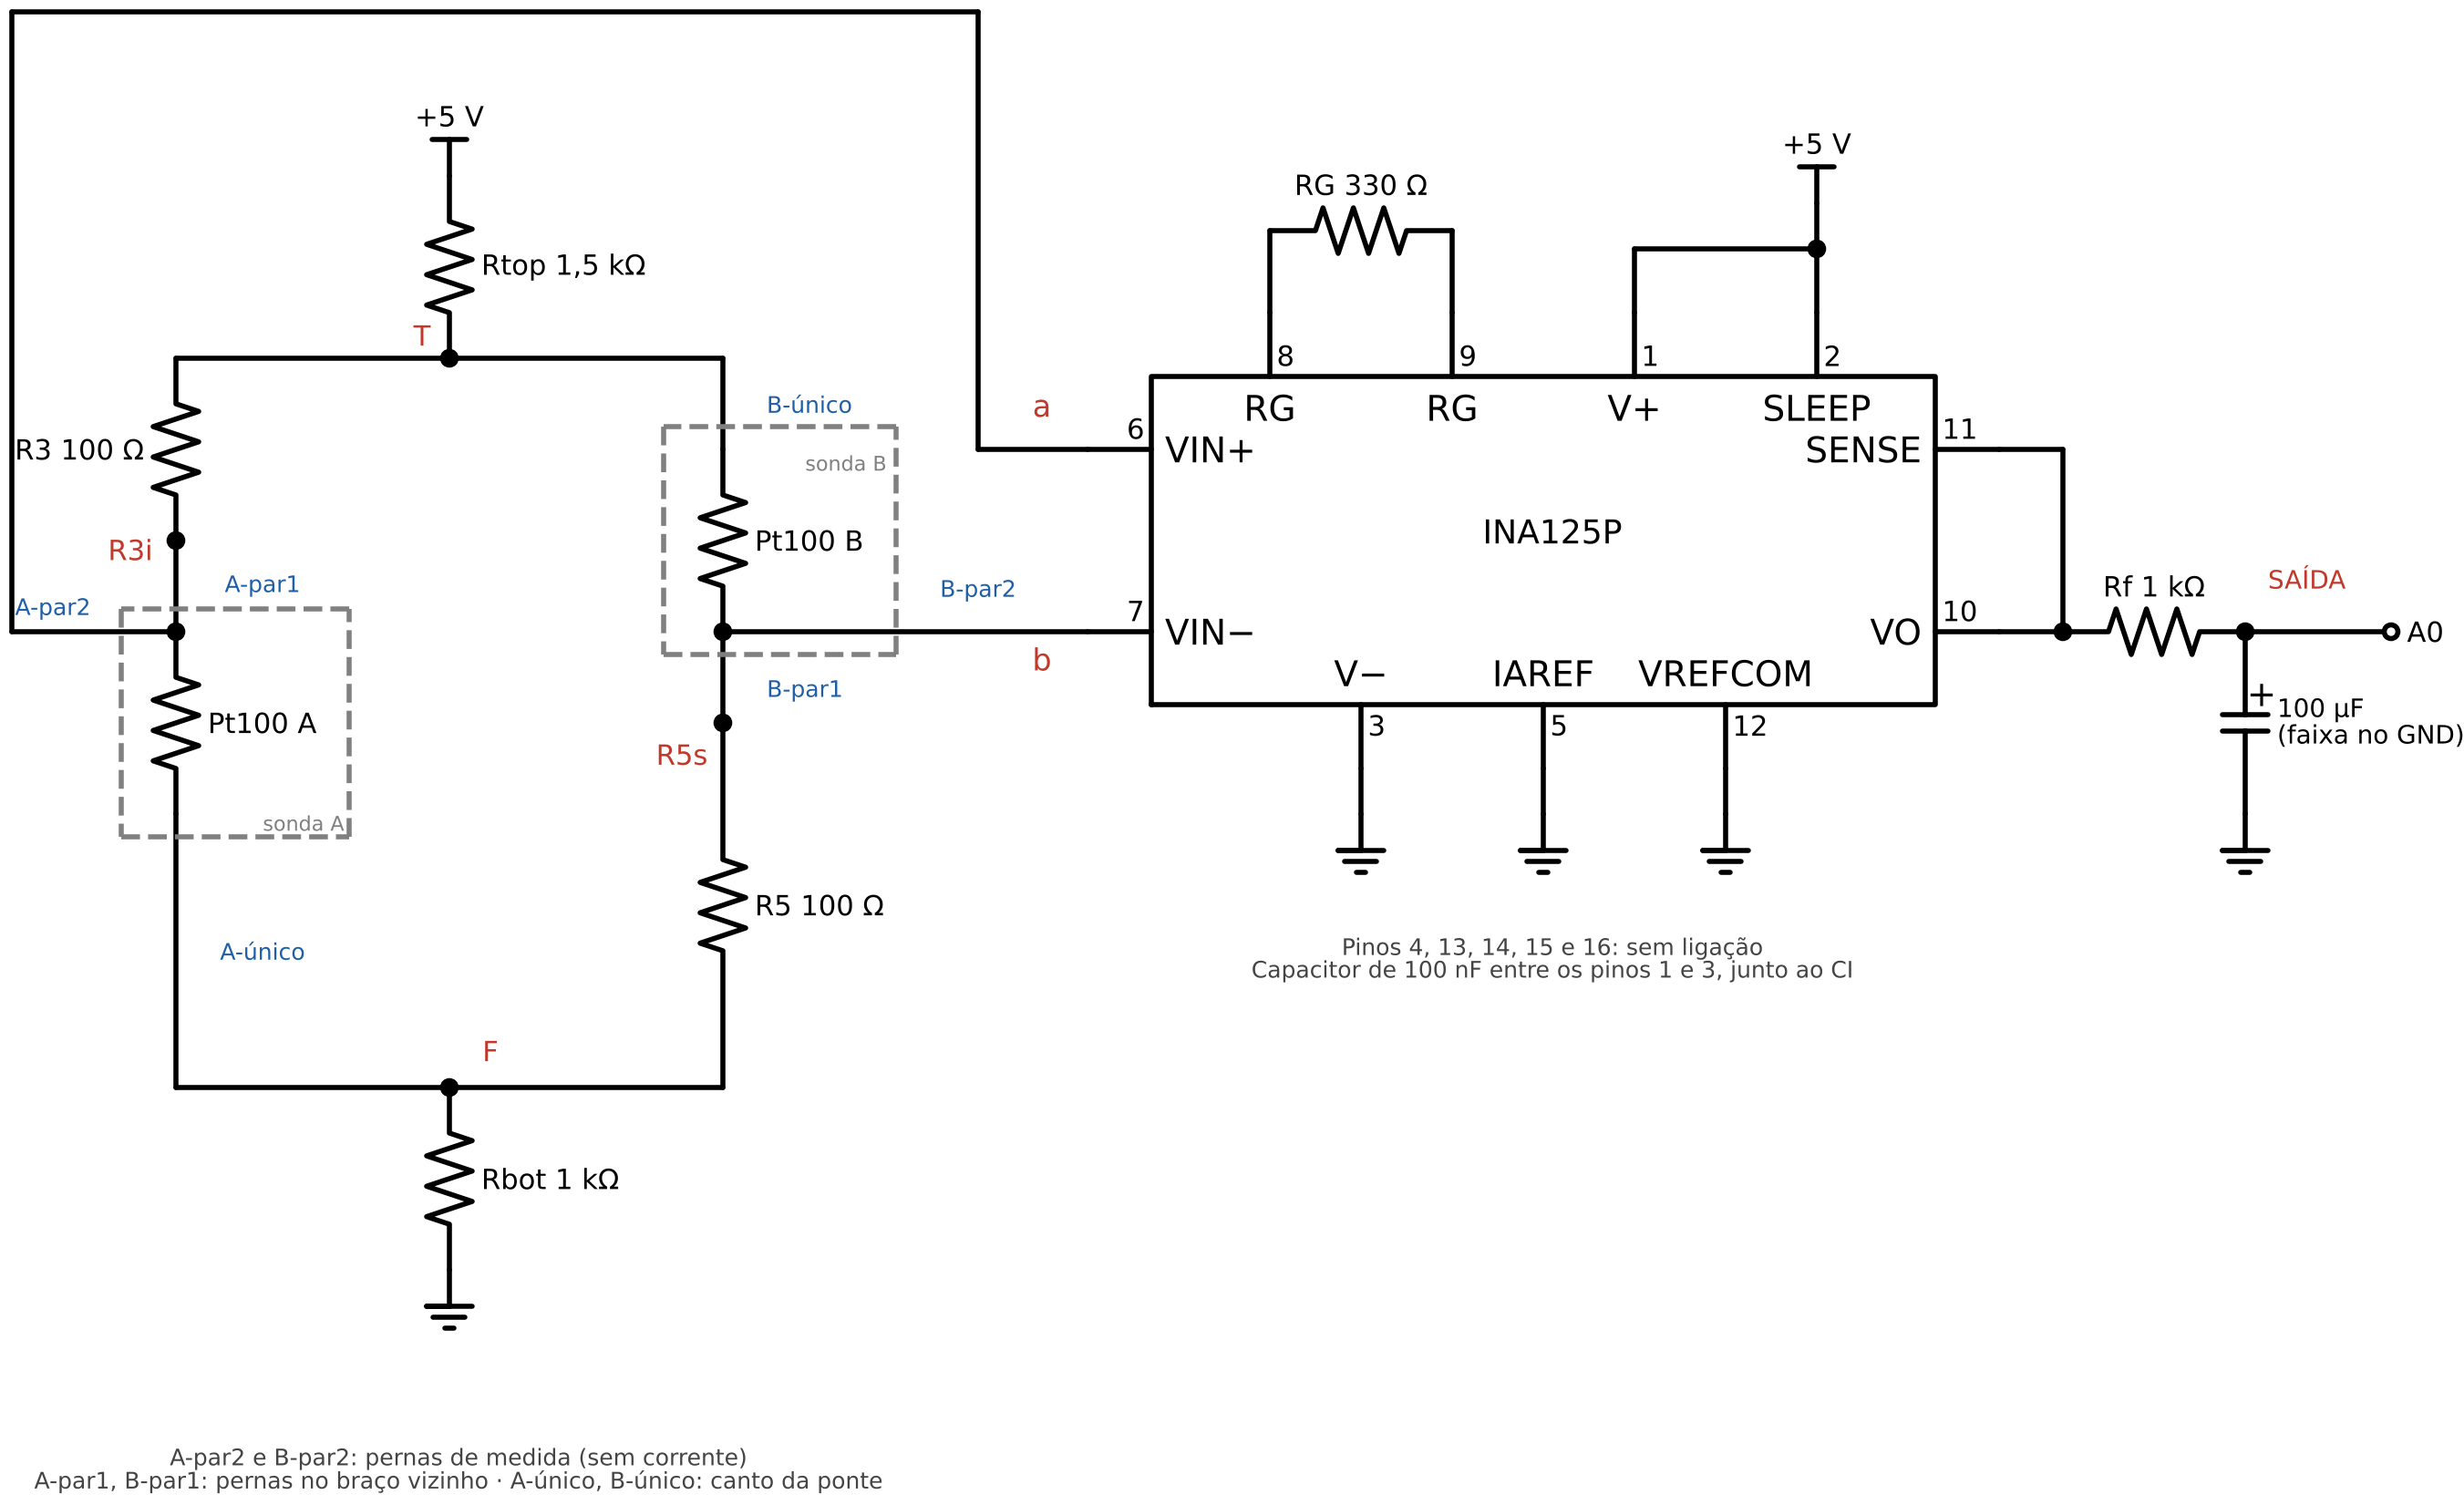
\includegraphics[width=\textwidth]{esq_pt100_ina125.png}
  \caption{Condicionamento dos Pt100: ponte de Wheatstone com dois sensores em braços opostos e ligação a 3 fios, amplificador de instrumentação INA125P e filtro anti-\textit{aliasing} na entrada A0.}
  \label{fig:esq_pt100}
\end{figure}

\paragraph{Ponte de Wheatstone.} Os dois Pt100 ficam em braços opostos da ponte, ambos dentro da câmara. Assim, quando a temperatura sobe, a tensão no nó $a$ aumenta e a do nó $b$ diminui, o que dobra a sensibilidade em relação a uma ponte com um único sensor. Os resistores de 100\,$\Omega$ equilibram a ponte em 0\,\ensuremath{^\circ}C.

\paragraph{Corrente nos sensores e modo comum.} Os resistores $R_{top}$ = 1,5\,k$\Omega$ e $R_{bot}$ = 1\,k$\Omega$ em série com a ponte limitam a corrente total a
\begin{equation}
  I = \frac{5}{1500 + 100 + 1000} \approx 1{,}92\ \text{mA},
\end{equation}
ou cerca de 0,96\,mA em cada Pt100. O autoaquecimento resultante ($I^2 R \approx 0{,}1$\,mW) é desprezível com a ventilação forçada. Esses resistores também posicionam as entradas do INA125P em aproximadamente 2,0\,V, dentro da faixa de modo comum do amplificador com alimentação única de 5\,V.

\paragraph{Sensibilidade e ganho.} Para pequenas variações de resistência, a saída da ponte é aproximadamente
\begin{equation}
  V_{ab} \approx I_{ramo}\,\Delta R = 0{,}96\ \text{mA} \times 0{,}385\ \Omega/{}^\circ\text{C} \approx 0{,}37\ \text{mV}/{}^\circ\text{C}.
\end{equation}
O ganho do INA125P é definido por $R_G$:
\begin{equation}
  G = 4 + \frac{60\ \text{k}\Omega}{R_G} = 4 + \frac{60\,000}{330} \approx 186,
\end{equation}
o que resulta em cerca de 69\,mV/\ensuremath{^\circ}C na saída e em uma resolução de aproximadamente 0,07\,\ensuremath{^\circ}C por LSB do conversor A/D. O pino SLEEP é ligado a V+, o pino SENSE à saída VO, e os pinos V$-$, IAREF e VREFCOM ao terra do Arduino. Os pinos da referência interna (4 e 13 a 16) não são utilizados.

\paragraph{Faixa de medição.} A saída do INA125P com alimentação única de 5\,V é considerada linear entre aproximadamente 0,8\,V e 4,2\,V. Com o ganho escolhido, isso corresponde à faixa de 12\,\ensuremath{^\circ}C a 61\,\ensuremath{^\circ}C, que cobre a faixa de operação prevista. Como a saída não ultrapassa a alimentação de 5\,V, a entrada do Arduino não precisa de diodos de proteção.

\paragraph{Ligação a 3 fios.} Cada Pt100 tem um par de fios ligado a uma das extremidades do sensor e um fio único ligado à outra. Em cada metade da ponte, a corrente percorre um fio do par, em série com o resistor de 100\,$\Omega$ do braço vizinho, e o fio único, em série com o próprio sensor. Como os dois braços de uma mesma metade recebem resistências de fio iguais, o efeito dos cabos se cancela com a ponte próxima do equilíbrio. O segundo fio do par leva a tensão do nó até a entrada do INA125P, que praticamente não drena corrente, de modo que a resistência desse fio não altera a medida.

\paragraph{Conversão e calibração.} Na faixa de 15\,\ensuremath{^\circ}C a 60\,\ensuremath{^\circ}C, o erro de não linearidade em relação a uma reta é de no máximo 0,11\,\ensuremath{^\circ}C (Seção~\ref{sec:simulacao}). A conversão de tensão em temperatura pode, portanto, ser linear. Como a tolerância de 1\,\% dos resistores da ponte gera um erro de offset de alguns graus, a reta será ajustada por calibração em dois pontos, comparando a leitura com um termômetro de referência.

\paragraph{Filtro.} O filtro RC na entrada A0, com $R_f$ = 1\,k$\Omega$ e $C_f$ = 100\,$\mu$F, tem constante de tempo de 0,1\,s e frequência de corte de
\begin{equation}
  f_c = \frac{1}{2\pi R_f C_f} \approx 1{,}6\ \text{Hz},
\end{equation}
muito acima da dinâmica térmica da câmara, que é da ordem de minutos. Ele atenua ruídos e o acoplamento do PWM. O resistor de 1\,k$\Omega$ também mantém baixa a impedância vista pelo conversor A/D.

% ================= 6 =================
\section{Medição da temperatura ambiente}

A temperatura ambiente é medida por um sensor DS18B20 em sonda de aço inoxidável à prova d'água, com cabo de 90\,cm. O DS18B20 é um sensor digital: o elemento sensor, o conversor A/D e a interface de comunicação estão integrados no próprio encapsulamento, e a leitura é transmitida ao Arduino pelo barramento 1-Wire. Por isso, o circuito externo se resume à alimentação, a um resistor de \textit{pull-up} e a um capacitor de desacoplamento (Figura~\ref{fig:esq_ds18b20}).

\begin{figure}[H]
  \centering
  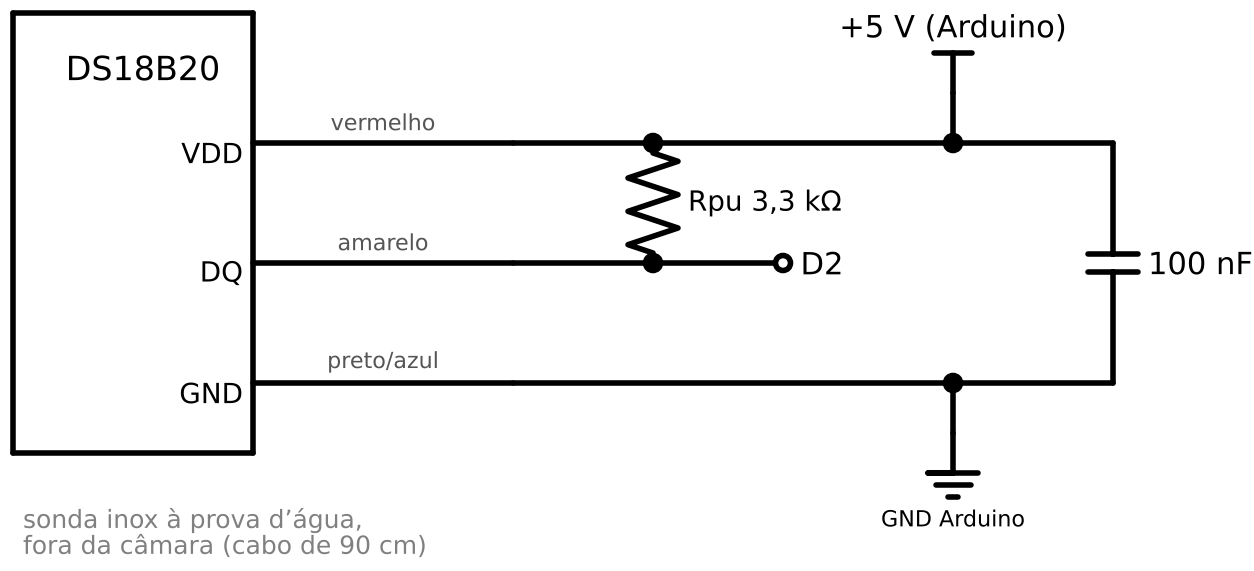
\includegraphics[width=0.75\textwidth]{esq_ds18b20.png}
  \caption{Ligação do sensor DS18B20 ao Arduino: alimentação em 5\,V, linha de dados (DQ) no pino digital D2 com resistor de \textit{pull-up} de 3,3\,k$\Omega$ e capacitor de desacoplamento de 100\,nF.}
  \label{fig:esq_ds18b20}
\end{figure}

\paragraph{Ligação.} O fio vermelho é ligado ao +5\,V, o fio de dados ao pino digital D2 e o fio de terra ao GND do Arduino. Como a sonda utilizada tem fios vermelho, azul e preto, o fio de terra é confirmado com o multímetro no modo diodo antes da primeira energização, já que a inversão entre alimentação e terra danifica o sensor. A linha de dados é de dreno aberto e precisa de um resistor de \textit{pull-up}; foi usado 3,3\,k$\Omega$, valor disponível no laboratório e adequado ao comprimento do cabo.

\paragraph{Características.} O sensor opera de $-$55 a 125\,\ensuremath{^\circ}C, com exatidão de $\pm$0,5\,\ensuremath{^\circ}C entre $-$10 e 85\,\ensuremath{^\circ}C. Com resolução de 12 bits, o passo de leitura é de 0,0625\,\ensuremath{^\circ}C e o tempo de conversão é de até 750\,ms. Como a temperatura ambiente varia em escala de minutos, uma leitura por segundo é suficiente para a compensação da perturbação. A conversão será disparada sem bloqueio (\textit{non-blocking}) pelas bibliotecas OneWire e DallasTemperature, de modo que a espera de 750\,ms não interrompa a malha de controle. Como a leitura é digital, ela não depende da referência do conversor A/D nem sofre interferência do PWM ao longo do cabo.

\paragraph{Posicionamento.} A sonda fica suspensa no ar a cerca de 20\,cm da câmara, longe da fonte e das passagens de cabos, para não medir o calor que escapa da câmara.

% ================= 7 =================
\section{Circuito de acionamento do aquecedor}
\label{sec:acionamento}

O circuito de acionamento é mostrado na Figura~\ref{fig:esq_acion}.

\begin{figure}[H]
  \centering
  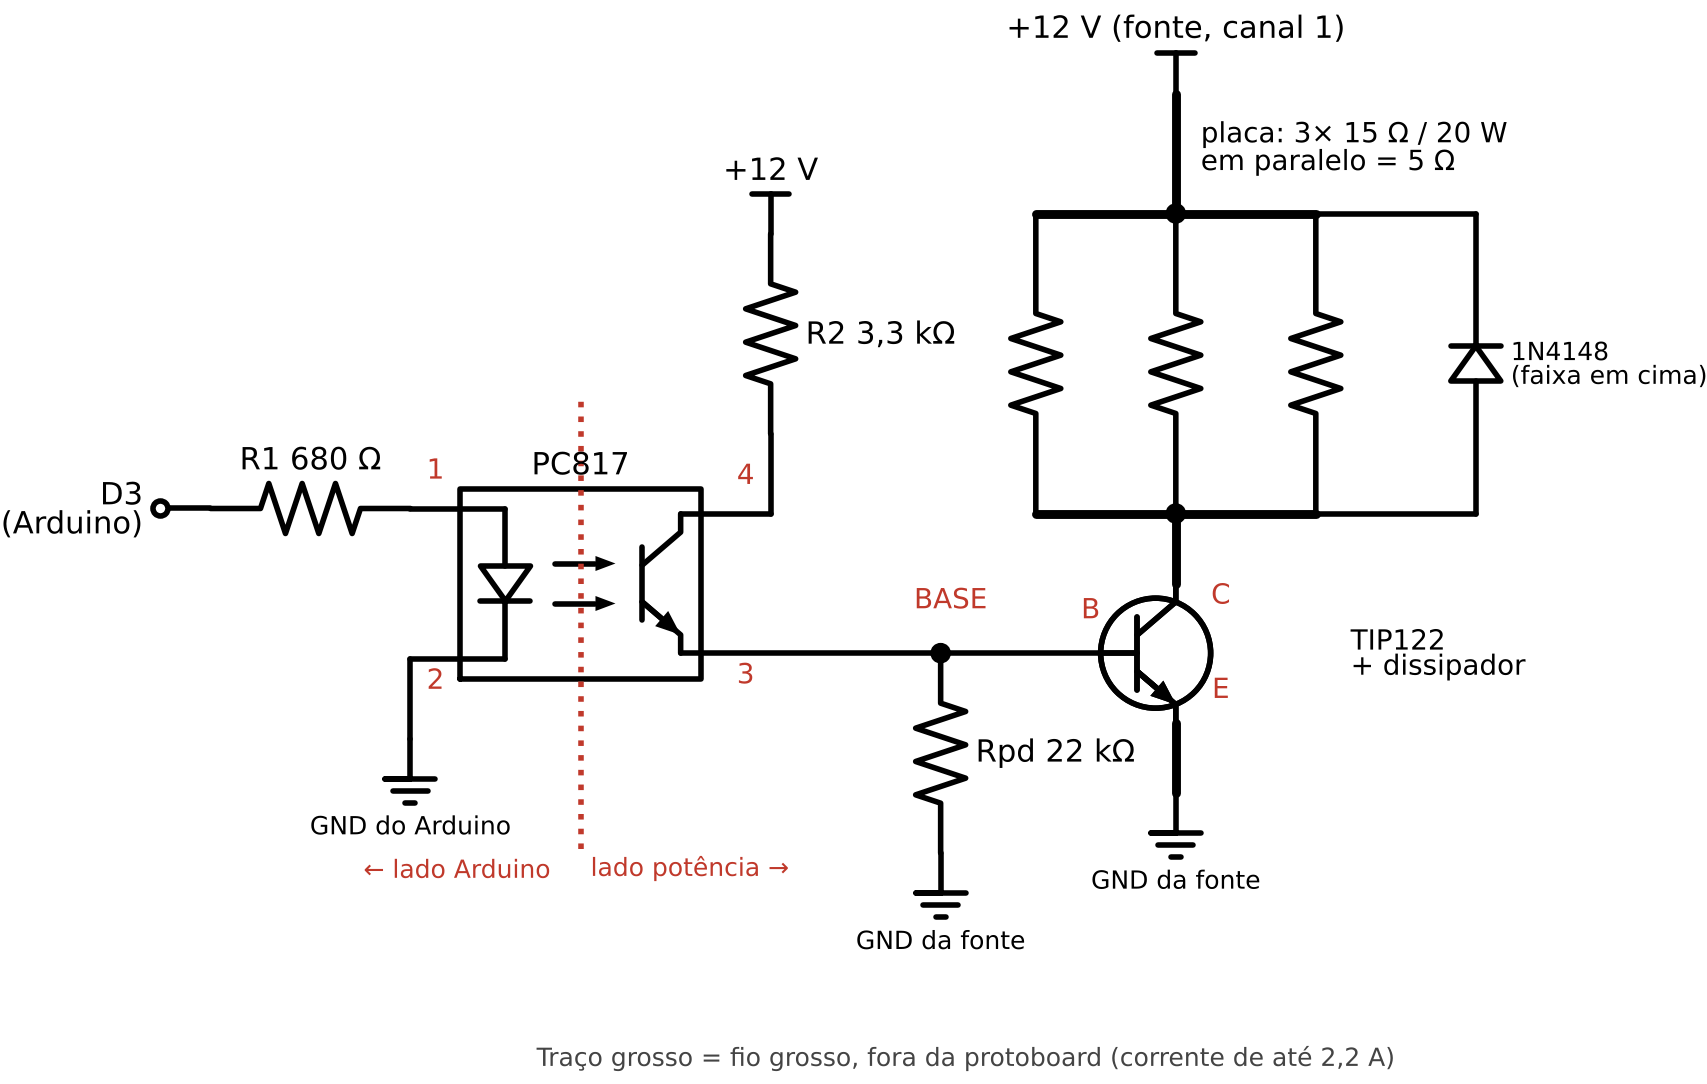
\includegraphics[width=0.9\textwidth]{esq_acionamento.png}
  \caption{Acionamento do aquecedor: optoacoplador PC817, transistor Darlington TIP122 e placa com três resistores de 15\,$\Omega$ em paralelo, alimentada em 12\,V. A linha pontilhada separa os dois lados isolados.}
  \label{fig:esq_acion}
\end{figure}

\paragraph{Optoacoplador.} O pino D3 do Arduino aciona o LED do PC817 por meio de $R_1$ = 680\,$\Omega$:
\begin{equation}
  I_F = \frac{5 - 1{,}2}{680} \approx 5{,}6\ \text{mA}.
\end{equation}
Considerando a razão de transferência de corrente (CTR) mínima de 50\,\%, o fototransistor conduz pelo menos 2,8\,mA. O resistor $R_2$ = 3,3\,k$\Omega$ ligado a 12\,V limita essa corrente a no máximo cerca de 3,1\,mA. O optoacoplador isola eletricamente o Arduino do circuito de potência, e cada lado tem a sua própria referência de terra.

\paragraph{TIP122.} Para a corrente de coletor de 2,2\,A e ganho mínimo $h_{FE} = 1000$, a corrente de base necessária é de
\begin{equation}
  I_B \geq \frac{2{,}2}{1000} \approx 2{,}2\ \text{mA},
\end{equation}
inferior aos cerca de 2,7\,mA fornecidos pelo optoacoplador no caso mais desfavorável, já descontada a corrente desviada pelo \textit{pull-down}. Como a folga é pequena, a saturação será verificada na montagem medindo $V_{CE}$; se passar de cerca de 2\,V, $R_1$ será reduzido para 330\,$\Omega$. O resistor de \textit{pull-down} de 22\,k$\Omega$ mantém o transistor em corte quando o optoacoplador está desligado, inclusive durante a inicialização do Arduino.

\paragraph{Dissipação.} Por ser um Darlington, o TIP122 saturado apresenta queda de tensão de aproximadamente 1,1\,V. A potência dissipada com PWM em 100\,\% é de cerca de $1{,}1 \times 2{,}2 \approx 2{,}5$\,W. Sem dissipador (resistência térmica junção-ambiente de 62,5\,\ensuremath{^\circ}C/W), a elevação de temperatura passaria de 150\,\ensuremath{^\circ}C. Por isso, o TIP122 é montado em um dissipador TO-220 com pasta térmica, que é obrigatório nesta aplicação. Como a aba do TIP122 é ligada ao coletor, o dissipador não pode encostar em outras partes metálicas.

\paragraph{Montagem do circuito de potência.} O caminho da corrente do aquecedor (fonte, placa, TIP122 e retorno) não passa pela protoboard, cujos contatos não suportam 2,2\,A com segurança. Ele é montado com fio de pelo menos 0,5\,mm$^2$ em uma barra de terminais, onde também é fixado o TIP122. Apenas a ligação da base vem da protoboard.

\paragraph{Proteções e PWM.} O diodo 1N4148 em antiparalelo com o aquecedor limita a sobretensão causada pela indutância parasita dos resistores no desligamento; a energia envolvida ($\tfrac{1}{2} L I^2 \approx 5\,\mu$J para $L \approx 2\,\mu$H) é pequena para o diodo. O protetor térmico KSD301, se disponível, fica em série com o aquecedor e interrompe a alimentação acima de 70\,\ensuremath{^\circ}C. O PWM padrão do pino D3 (490\,Hz) é adequado, pois a dinâmica térmica é muito mais lenta que o período de chaveamento. A ventoinha é alimentada diretamente pelo canal 2 da fonte, em 12\,V, e opera com rotação constante.

{\color{red}\noindent\textbf{[A FAZER: refazer as simulações no LTspice com os componentes finais (arquivos em \texttt{simulacoes\_ltspice\_final.zip}): novo print do esquemático do circuito 1 e novos prints do esquemático e das formas de onda do circuito 2. Os números do texto já correspondem aos componentes finais.]}}

% ================= 8 =================
\section{Validação por simulação}
\label{sec:simulacao}

Os circuitos foram simulados no LTspice. O INA125P foi representado pela sua topologia interna de três amplificadores operacionais, o TIP122 por um par Darlington com os resistores internos do componente e o PC817 por um LED acoplado a um fototransistor com CTR de 50\,\%, o caso mais desfavorável.

\subsection{Medição da temperatura interna}

O circuito da Figura~\ref{fig:lt_esq_pt100} foi simulado com a temperatura dos dois Pt100 variando de 0 a 100\,\ensuremath{^\circ}C. Os sensores foram modelados pela equação de Callendar--Van Dusen, e a resistência de cada fio ($R_L$) foi considerada igual a 0,1\,$\Omega$, incluindo os fios de medida que levam a tensão até o INA125P. Os resultados estão na Figura~\ref{fig:lt_sim_pt100} e na Tabela~\ref{tab:sim_pt100}.

\begin{figure}[H]
  \centering
  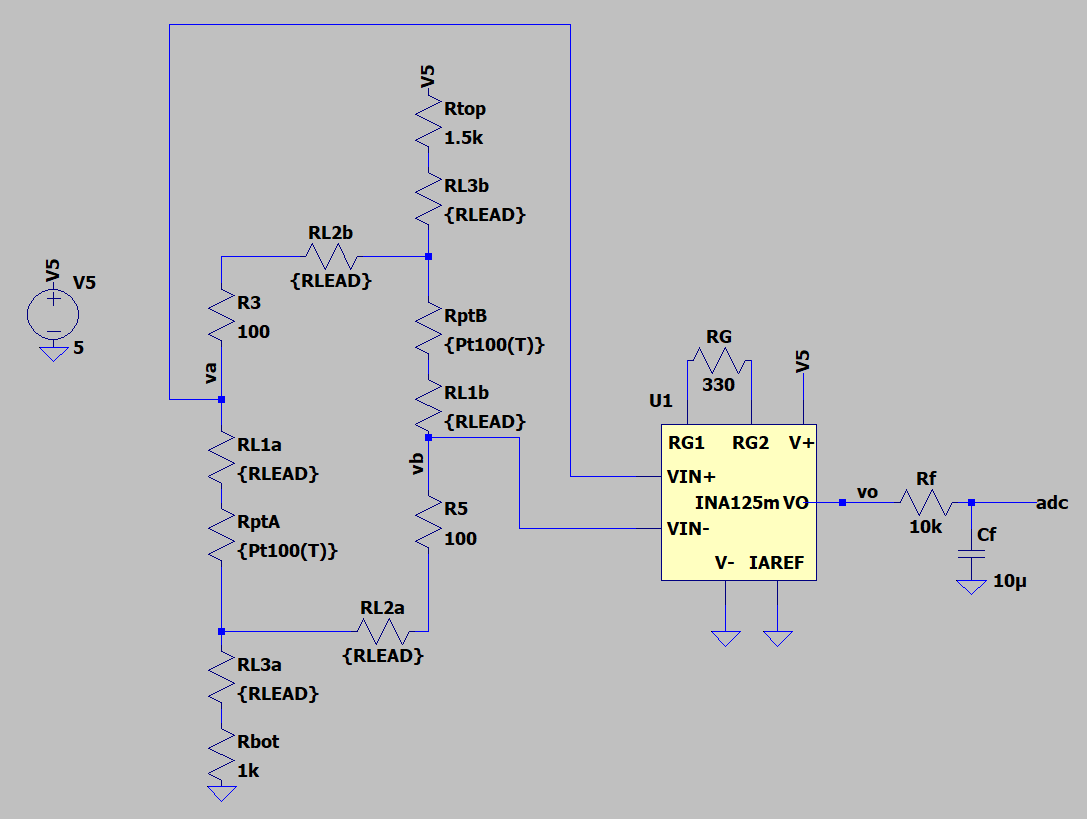
\includegraphics[width=0.85\textwidth]{lt_esq_pt100.png}
  \caption{Circuito de medição da temperatura interna simulado no LTspice, com as resistências dos fios dos Pt100 representadas explicitamente.}
  \label{fig:lt_esq_pt100}
\end{figure}

\begin{figure}[H]
  \centering
  \begin{subfigure}{\textwidth}
    \centering
    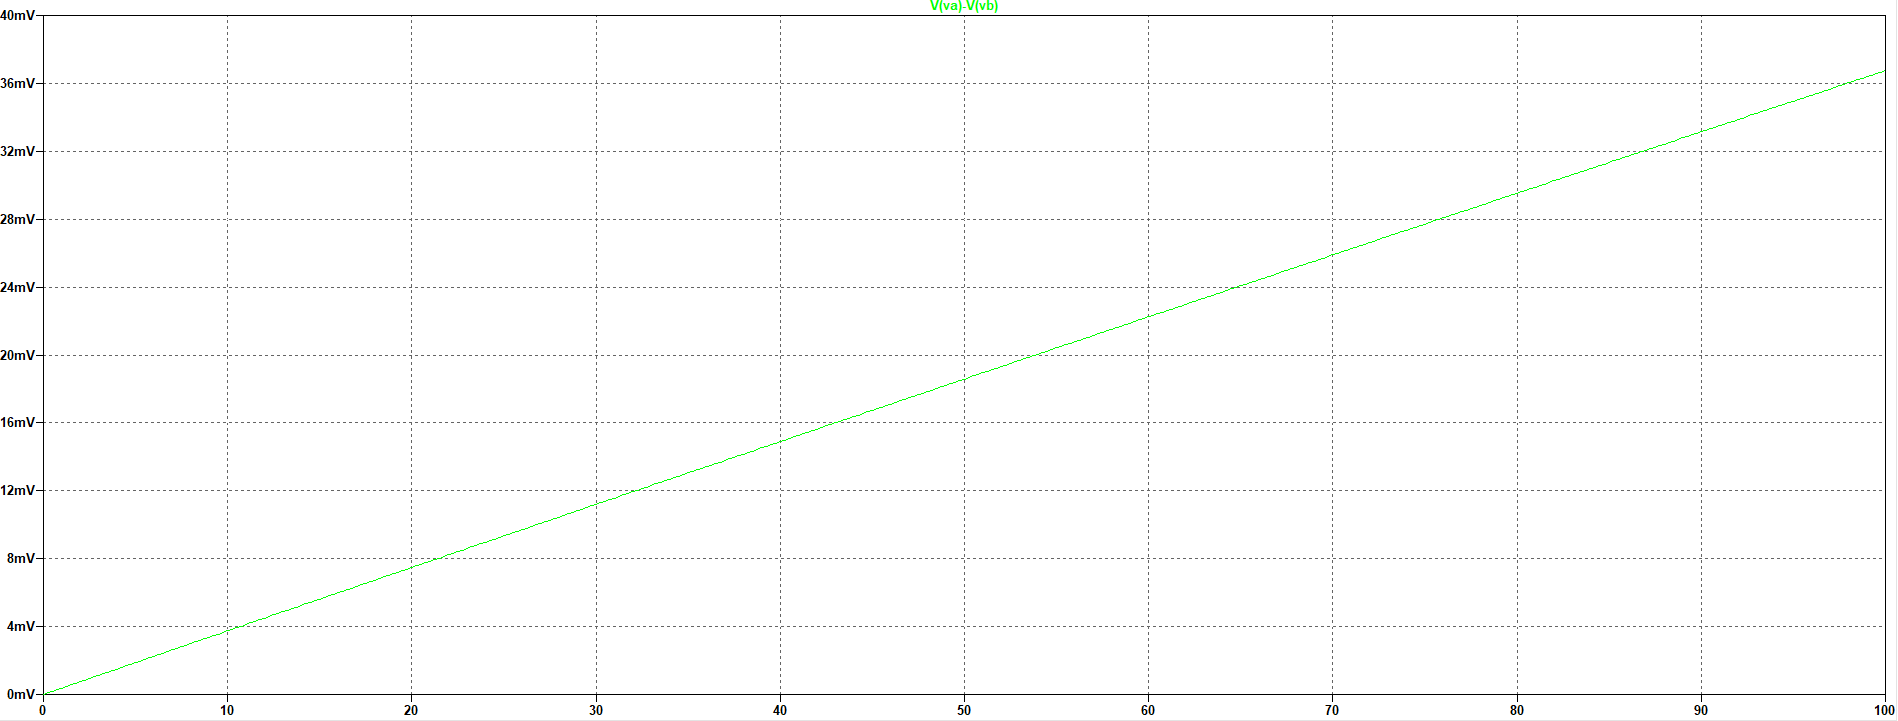
\includegraphics[width=\textwidth]{lt_vab_pt100.png}
    \caption{Saída da ponte de Wheatstone, $V_{ab} = V_a - V_b$.}
  \end{subfigure}
  \vspace{0.3cm}
  \begin{subfigure}{\textwidth}
    \centering
    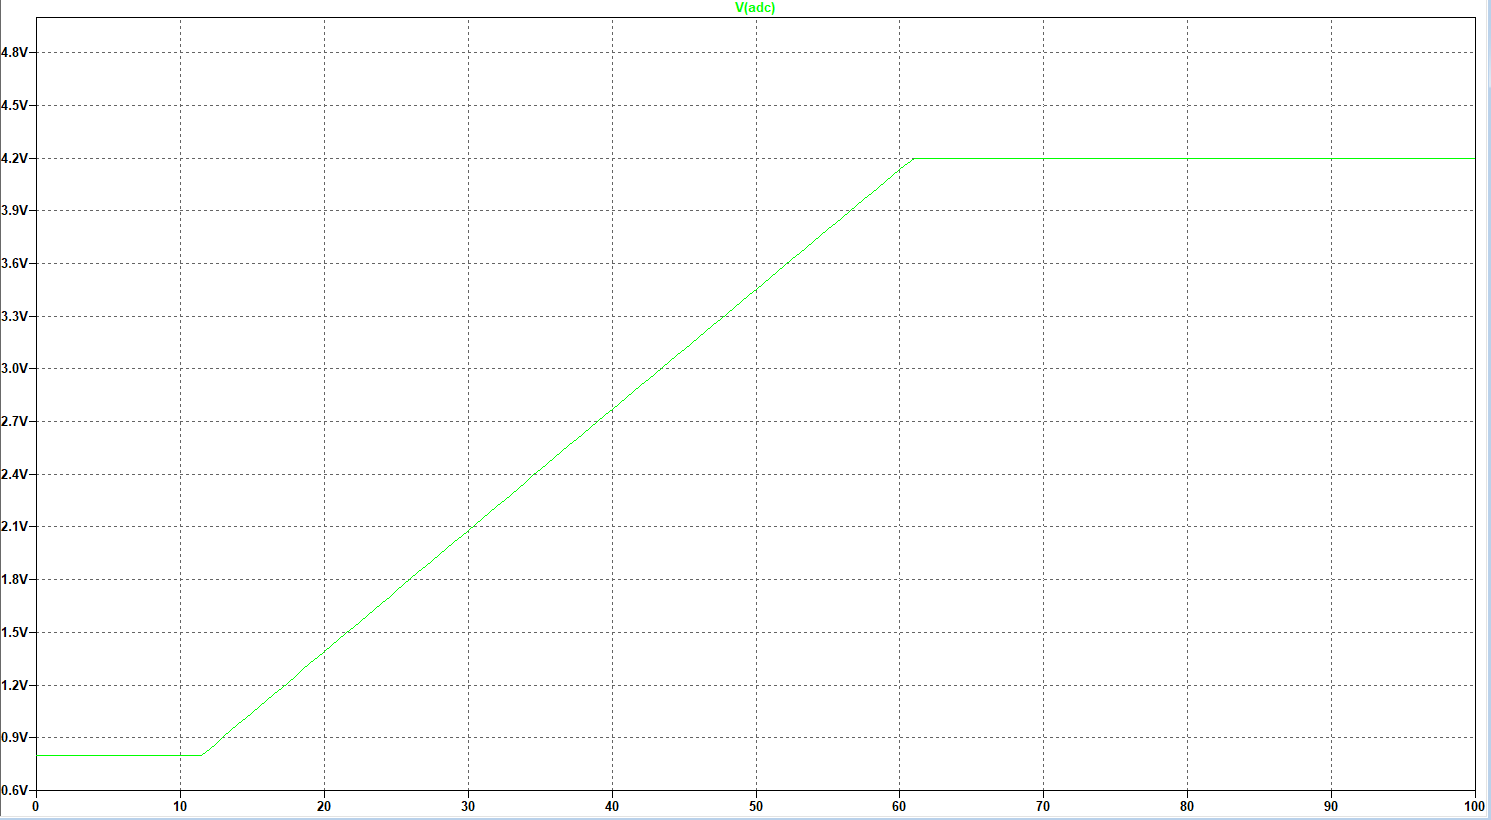
\includegraphics[width=\textwidth]{lt_vadc_pt100.png}
    \caption{Saída do INA125P após o filtro (entrada A0 do Arduino).}
  \end{subfigure}
  \caption{Resultados da simulação da medição interna. O eixo horizontal corresponde à temperatura dos Pt100, em \ensuremath{^\circ}C.}
  \label{fig:lt_sim_pt100}
\end{figure}

\begin{table}[H]
\centering
\small
\renewcommand{\arraystretch}{1.2}
\caption{Resultados simulados da medição interna.}
\label{tab:sim_pt100}
\begin{tabular}{cccc}
\toprule
\textbf{T (\ensuremath{^\circ}C)} & \textbf{$V_{ab}$ (mV)} & \textbf{$V_{out}$ (V)} & \textbf{Contagens do A/D} \\
\midrule
15 & 5,62  & 1,044 & 214 \\
20 & 7,48  & 1,390 & 284 \\
25 & 9,34  & 1,736 & 355 \\
30 & 11,20 & 2,081 & 426 \\
40 & 14,90 & 2,768 & 566 \\
50 & 18,58 & 3,452 & 706 \\
60 & 22,25 & 4,134 & 846 \\
\bottomrule
\end{tabular}
\end{table}

Os principais resultados são:
\begin{itemize}
  \item sensibilidade de 68,7\,mV/\ensuremath{^\circ}C e resolução de 0,071\,\ensuremath{^\circ}C por LSB;
  \item faixa útil de 12\,\ensuremath{^\circ}C a 61\,\ensuremath{^\circ}C, limitada pela excursão de saída do INA125P;
  \item erro de não linearidade de no máximo 0,11\,\ensuremath{^\circ}C entre 15 e 60\,\ensuremath{^\circ}C, o que justifica a conversão linear;
  \item com resistência exagerada de 1\,$\Omega$ em cada fio, o erro foi de apenas $-$0,02\,\ensuremath{^\circ}C a 50\,\ensuremath{^\circ}C com a ligação a 3 fios, contra +5,2\,\ensuremath{^\circ}C em uma ligação a 2 fios equivalente.
\end{itemize}

\subsection{Acionamento}

O circuito da Figura~\ref{fig:lt_esq_acion} foi simulado com PWM de 490\,Hz e razão cíclica de 50\,\%. A indutância parasita dos resistores de aquecimento foi representada por $L_{heat}$ = 2\,$\mu$H. O terra do Arduino (\textit{gard}) é isolado do terra da fonte pelo optoacoplador; o resistor $R_{gnd}$ existe apenas para que o simulador tenha uma referência comum. As formas de onda são apresentadas na Figura~\ref{fig:lt_formas_acion}.

\begin{figure}[H]
  \centering
  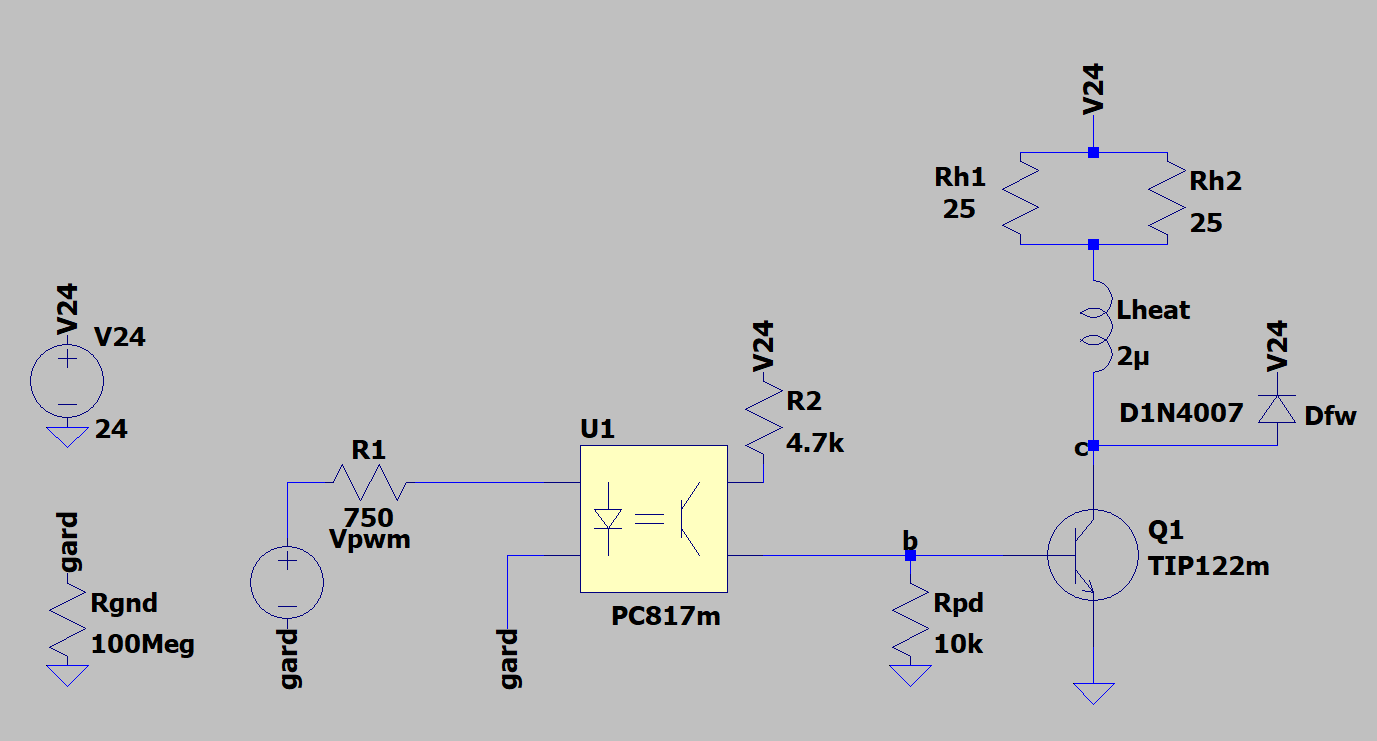
\includegraphics[width=0.9\textwidth]{lt_esq_acion.png}
  \caption{Circuito de acionamento simulado no LTspice: optoacoplador PC817, transistor Darlington TIP122 e placa com três resistores de 15\,$\Omega$ em paralelo, alimentada em 12\,V.}
  \label{fig:lt_esq_acion}
\end{figure}

\begin{figure}[H]
  \centering
  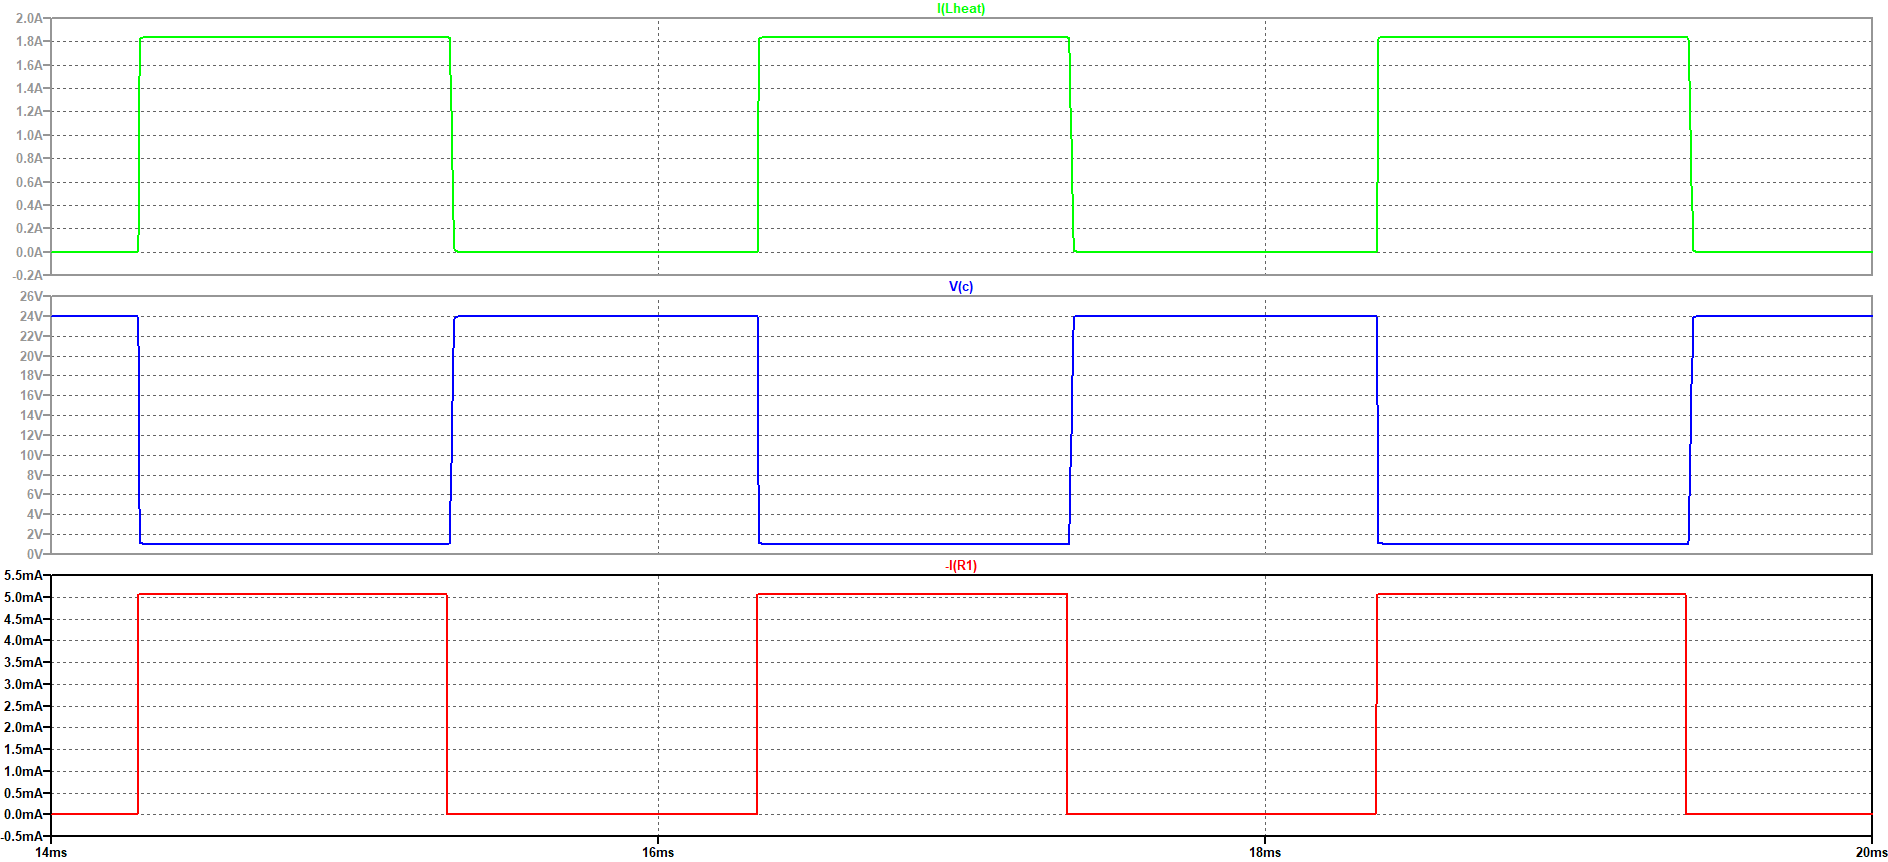
\includegraphics[width=\textwidth]{lt_formas_acion.png}
  \caption{Formas de onda simuladas do acionamento (PWM de 490\,Hz, D = 50\,\%): corrente no aquecedor, tensão no coletor do TIP122 e corrente no LED do PC817.}
  \label{fig:lt_formas_acion}
\end{figure}

Os principais resultados são:
\begin{itemize}
  \item corrente de 2,17\,A no aquecedor durante a condução, com o TIP122 saturado ($V_{CE} \approx 1{,}13$\,V);
  \item corrente de 5,6\,mA no LED do PC817 e cerca de 2,7\,mA na base do TIP122, acima do mínimo de 2,2\,mA necessário para a saturação;
  \item potência média de 12,2\,W no aquecedor e de 1,3\,W no TIP122 com razão cíclica de 50\,\%, ou seja, cerca de 24\,W e 2,6\,W em 100\,\%;
  \item tensão máxima de 12,1\,V no coletor durante o desligamento, limitada pelo diodo de roda livre.
\end{itemize}

% ================= 9 =================
\section{Esboço da estrutura mecânica}

O esboço da estrutura mecânica é apresentado na Figura~\ref{fig:mecanica}.

\begin{figure}[H]
  \centering
  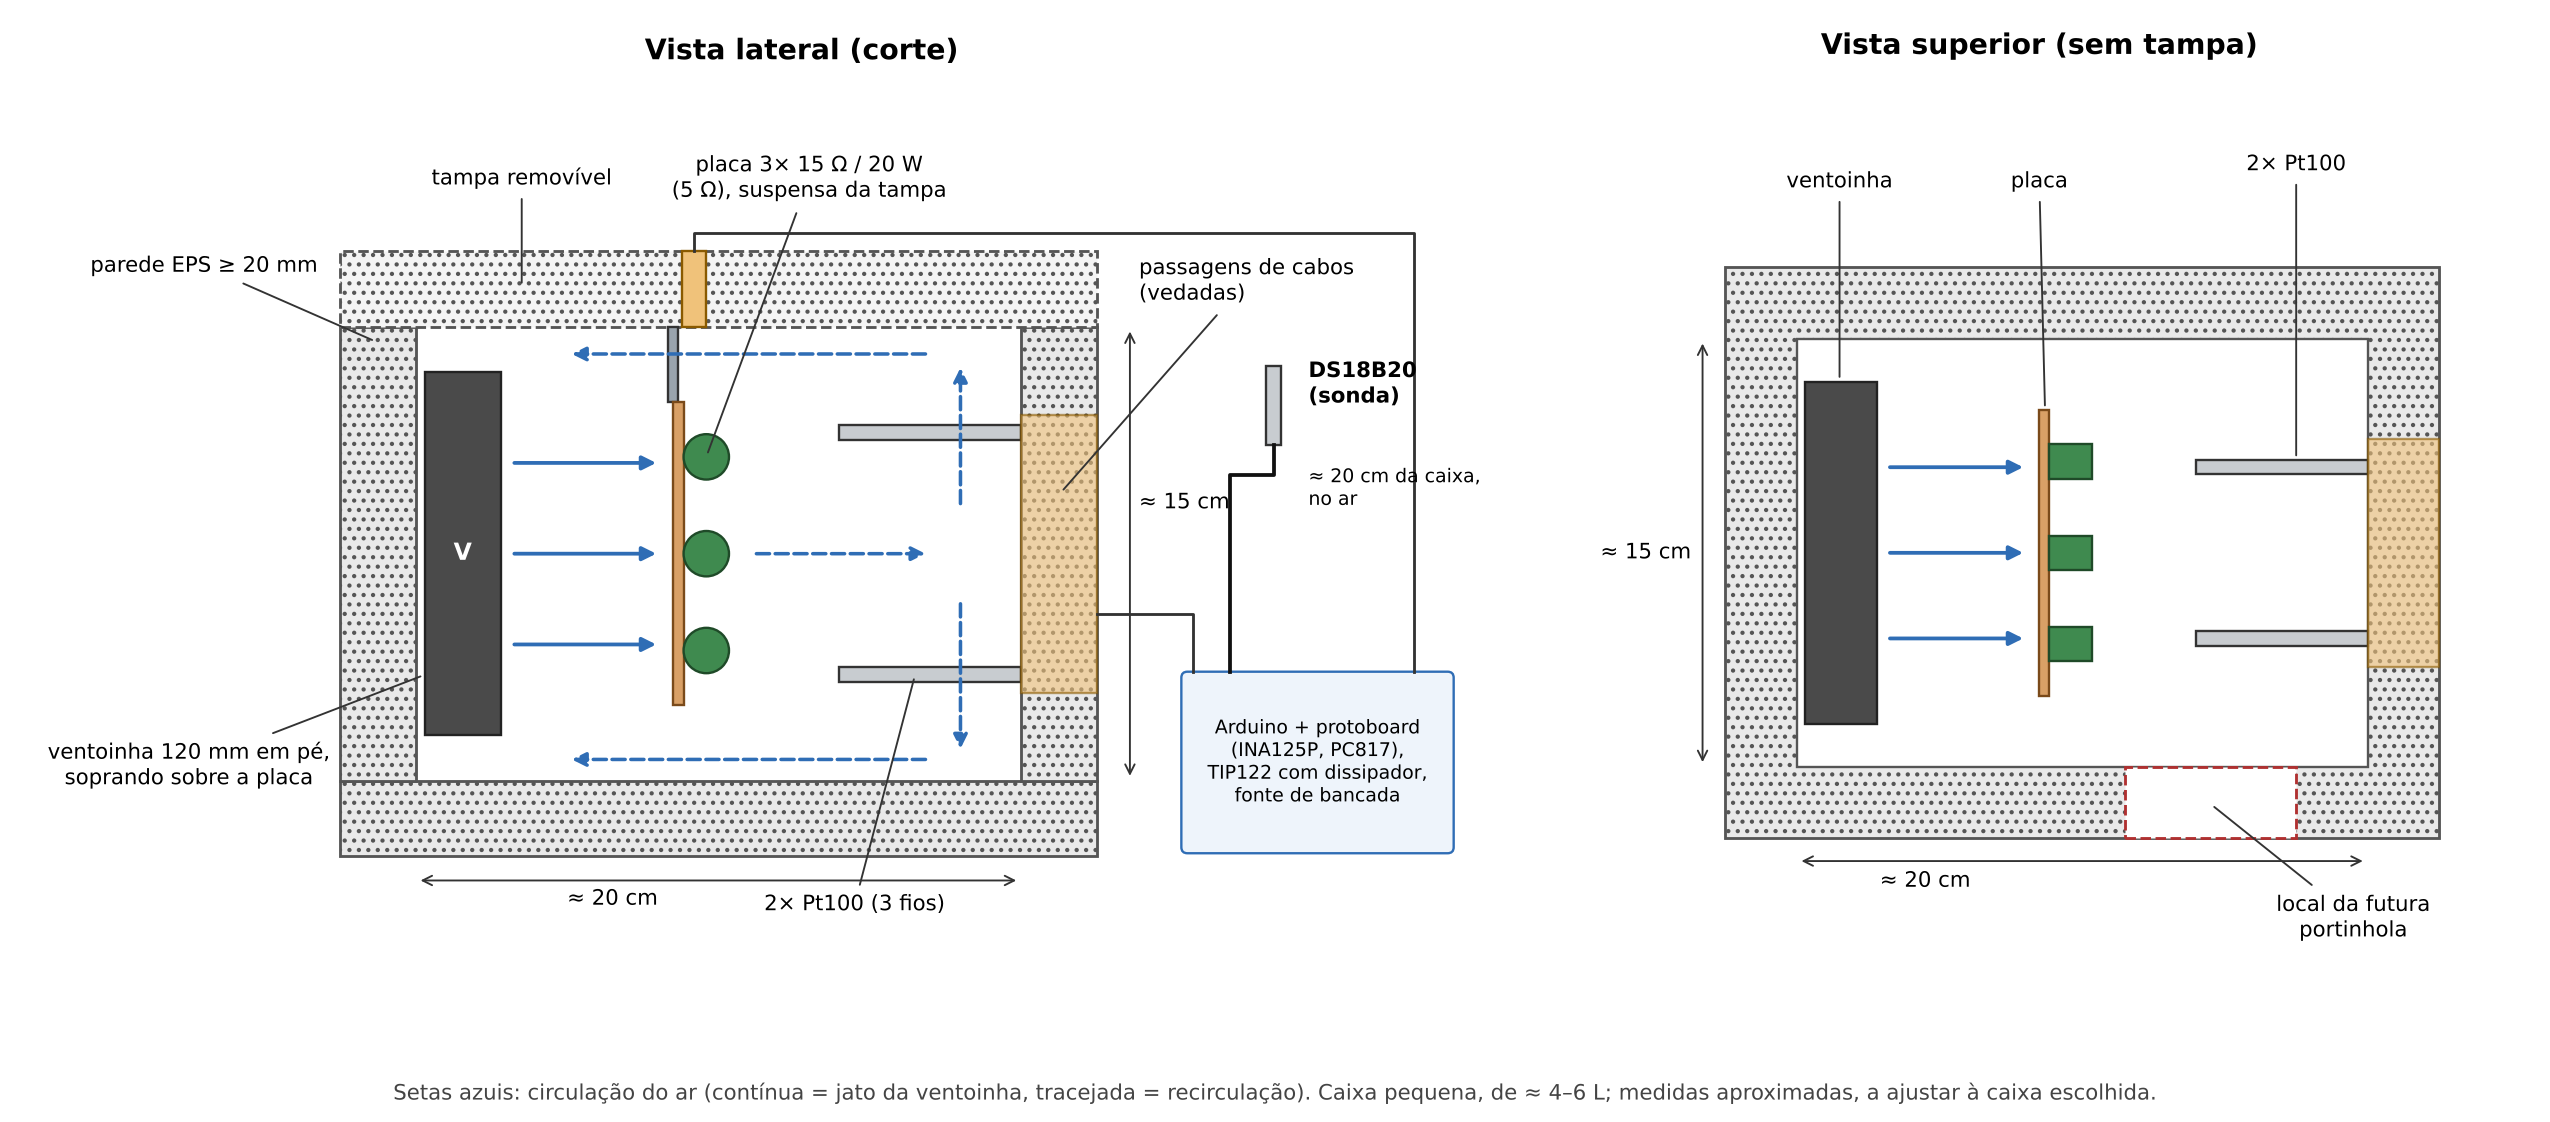
\includegraphics[width=\textwidth]{esboco_mecanico.png}
  \caption{Esboço da estrutura mecânica da câmara térmica: vista lateral em corte e vista superior sem tampa (medidas aproximadas).}
  \label{fig:mecanica}
\end{figure}

\begin{itemize}
  \item \textbf{Câmara:} caixa de EPS pequena, com tampa removível e dimensões internas da ordem de 20\,$\times$\,15\,$\times$\,15\,cm (cerca de 4 a 6\,L), a serem ajustadas à caixa escolhida. As paredes têm pelo menos 20\,mm.
  \item \textbf{Aquecedor:} a placa com os três resistores fica suspensa por um suporte metálico preso à tampa, sem encostar no EPS, com folga de alguns centímetros até as paredes. Os cabos de alimentação saem por um furo na tampa.
  \item \textbf{Ventoinha:} a ventoinha de 120\,mm fica em pé junto a uma parede lateral, soprando o ar diretamente sobre os resistores. O ar aquecido recircula pela tampa, pelo fundo e pelas paredes.
  \item \textbf{Pt100:} os dois sensores entram pela parede oposta, a alguns centímetros da placa, para medir a temperatura do ar da câmara e não a superfície dos resistores.
  \item \textbf{Fora da câmara:} ficam a sonda DS18B20, o Arduino, a protoboard com os circuitos, o TIP122 com dissipador na barra de terminais e a fonte de bancada. As passagens de cabos são vedadas com cola quente.
  \item \textbf{Perturbação:} uma das paredes tem previsto o local de uma futura portinhola, que poderá ser aberta para gerar perturbações nas próximas etapas. A segunda ventoinha disponível poderá soprar ar ambiente por essa abertura.
\end{itemize}


\end{document}
